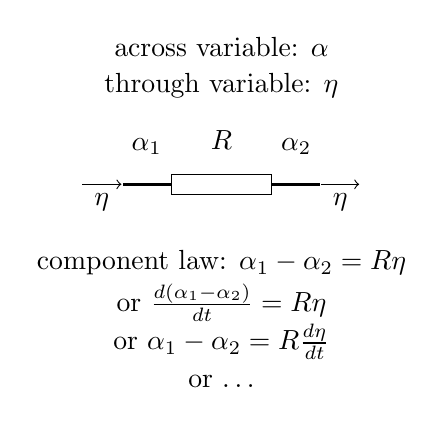
\begin{tikzpicture}
\draw (.75 , 1.75) node {across variable: $\alpha$};
\draw (.75, 1.25) node{through variable: $\eta$};
\draw (.75,0) node[rectangle,draw,minimum width=.5in,minimum height=.1in] (e) {};
\draw[very thick] (-.5,0) -- (e.180);
\draw[very thick] (e.0) -- (2,0);
\draw (.75,0) node[above=9pt] {$R$};
\draw (-.2,.25) node[above] {$\alpha_{1}$};
\draw[<-] (-.52,0) -- node[below] {$\eta$} ++(-.5,0);
\draw[->] (2.02,0) -- node[below] {$\eta$} ++(.48,0);
\draw (1.7,.25) node[above] {$\alpha_{2}$};
\draw (.75,-1) node {component law: $\alpha_{1}-\alpha_{2} = R\eta$};
\draw (.75,-1.5) node {or $\frac{d(\alpha_{1}-\alpha_{2})}{dt} = R\eta$};
\draw (.75,-2) node {or $\alpha_{1}-\alpha_{2} = R\frac{d\eta}{dt}$};
\draw (.75,-2.5) node {or $\dots$};
\end{tikzpicture}